\documentclass[uplatex,9pt,a5j]{jsarticle}

\pagestyle{plain}

\usepackage[top=5truemm,bottom=5truemm,left=10truemm,right=10truemm]{geometry}
\usepackage[dvipdfmx]{graphicx}
\usepackage{amsmath}
\usepackage{ascmac}
\usepackage{url}

\begin{document}

\section{ベイズモデリングで男子プロテニスの強さ分析}
 筆者はテニスが大好きで, ほとんどの週末はテニスを楽しんでいるし, 男子プロテニスの試合を見るのも好きである。男子プロテニスの世界ランキングのポイントは, ツアーを回った時の戦績によって決まるが, 勝った時に貰えるポイントは大会のレベルごとに異なっている。プレイヤーが一年間のツアーをどのように回るかもポイントに影響されるし, 出場条件のある大会もある。大会のトーナメント表のオーダー次第では, 中々勝ち上がれない選手もいたりする。こうした様々な要素から, 視聴者が見ていて感じるプレイヤーの強さと, 実際のランキングの順位の関係には, 時々違和感を感じることがある。\\
 本章では, ツアーの中での各プレイヤーごとの勝敗の結果のみを用いて, プレイヤーの強さをベイズモデリングしてみて, 違和感のない結果が得られるか試してみようと思う。なお, 分析を行なった時期が本章の執筆時期よりも期間が空いており, 最新の勝敗のデータを使った分析ではないことに留意していただきたいと共に, 興味のある読者がいれば, ぜひ最新のデータで試していただければと思う。\\

\subsection{本章で扱うデータ}
 本章では, ATPツアーの勝敗結果のデータセットが作成・公開されている\footnote{\url{https://github.com/JeffSackmann/tennis_atp.git}}ので, これを利用する。データセット作成者に感謝する。\\
 データセットの中身は, 1レコードが1試合を表しており, その試合のツアー名, ツアーレベル, 開催年月日, サーフェス, 何回戦か, 勝った選手の情報と得点, 負けた選手の情報と得点などが格納されている。Dockerで分析環境のコンテナを作る際に, GitHubをクローンするコマンドも入れておけば, そのデータセットを利用した分析環境のコンテナを用意することができる。\\

\subsection{プロテニスプレイヤーの強さのモデル}
\subsubsection{モデルの仮定}
 今回はツアーの中での各プレイヤーの直接対決の勝敗結果から, 各プレイヤーの強さをモデリングしてみる。\\
 具体的には, 松浦, 2016\footnote{松浦健太郎 (2016). Wonderful R 2 StanとRでベイズ統計モデリング 共立出版}で提案されている統計モデル(1)を利用する。\\
\begin{eqnarray}
  performance_{g,1} & {\sim} & Normal(\mu_{loser}, {\sigma_{pf}}_{loser}), \hspace{1em} g=1{\ldots}G \nonumber \\
  performance_{g,2} & {\sim} & Normal(\mu_{winner}, {\sigma_{pf}}_{winner}), \hspace{1em} g=1{\ldots}G \nonumber \\
  performance_{g,1} & < & performance_{g,2}, \hspace{1em} g=1{\ldots}G \\
  \mu_n & {\sim} & Normal(0,\sigma_{\mu}), \hspace{1em} n=1{\ldots}N \nonumber \\
  {\sigma_{pf}}_n & {\sim} & Gamma(10,10), \hspace{1em} n=1{\ldots}N \nonumber
  \label{eq:eq_model_strength}
\end{eqnarray}
 プレイヤー $n$ の強さを $\mu_n$ , 勝負ムラを ${\sigma_{pf}}_n$ として, 1回の勝負 $g$ で発揮する力(パフォーマンス)は, 平均 $\mu_n$, 勝負ムラ ${\sigma_{pf}}_n$ の正規分布から生成されると考える。ここで $loser$ は負けたプレイヤーのインデックス, $winner$ は勝ったプレイヤーのインデックスを表す。\\
 つまり, 各プレイヤーはそれぞれの強さの値を持っているが, 試合ごとに, 調子が良くてパフォーマンスを発揮できた時もあれば, 不調でパフォーマンスを発揮できなかった時などがあると考え, その変化の大きさをパフォーマンス発揮のムラとして考える。そして, 勝負の結果はパフォーマンスの大小で決まる、つまり、大きかった方が勝つと考える。\\
 統計モデル(1)をStanコードで表すと, 付録()の通りとなる。\\
 コード内の \verb|ordered[2] performance[G];| がこのモデルでの重要なところで, 制約付きパラメータと呼ばれる。ここもう少し追加する。\\
 データの対象期間は, 2015.01〜2017.02の戦績データを利用した。\\
 対象プレイヤーは, この期間中の戦績データ数を確認しながら手動で選択した。今回は完全に個人的な興味と, データ数の兼ね合いで, 以下のプレイヤーのリストを用意した。(敬称略)\\
\begin{table}[htb]
  \begin{tabular}{lll}
    Roger Federer & Milos Raonic & Richard Gasquet \\
    Rafael Nadal & Kei Nishikori & Marin Cilic \\
    Novak Djokovic & Gael Monfils & Grigor Dimitrov \\
    Andy Murray & Tomas Berdych & Dominic Thiem \\
    Stanislas Wawrinka & Jo Wilfried Tsonga & Nick Kyrgios \\
    Juan Martin Del Potro & David Ferrer & Alexander Zverev \\
  \end{tabular}
\end{table}
 お馴染みのBIG4\footnote{男子シングルスプロテニスにおいて, 特に優秀な成績を収めている Roger Federer, Rafael Nadal, Novak Djokovic, Andy Murray の4選手の総称}に加えて, Kei Nishikori, Juan Martin Del Potro, Milos Raonic などの中堅, Tomas Berdych, Jo Wilfried Tsonga, David Ferrer など, 昔からTOP10付近に位置しているプレイヤー, そして若手プレイヤーとして活躍してきている Dominic Thiem, Nick Kyrgios, Alexander Zverev などを入れてみた。\\

\subsubsection{プロテニスプレイヤーの強さの推定結果と考察}
 収束の確認については, Rhat統計量が1.1以下であることを確認し, 各チェインごとのサンプリングプロットが違和感なく重なるかなども確認した。\\
 まずは各プレイヤーの強さ $\mu_n$ の事後分布が図*,  表*の通りである。\\
\begin{figure}[htbp]
  \begin{center}
    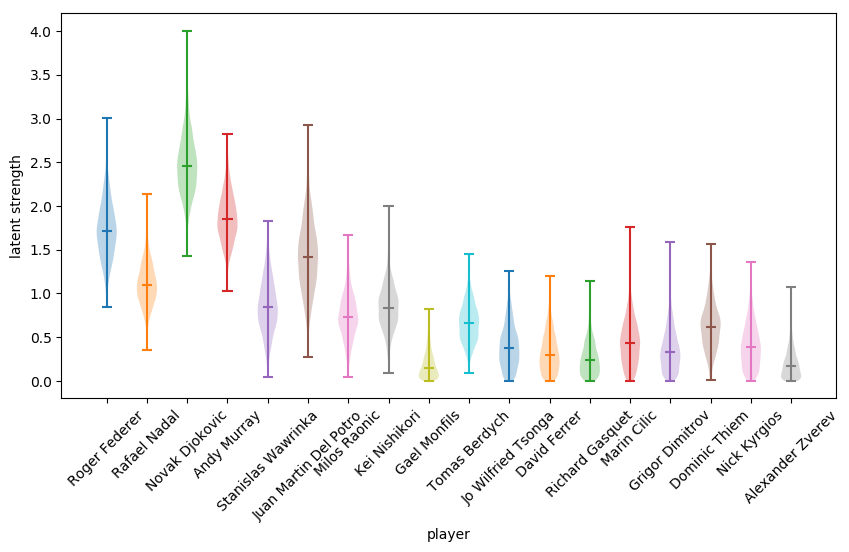
\includegraphics[clip,width=12.0cm]{./graphs/strength_mu.png}
    \caption{各プレイヤーの強さ $\mu_n$ の事後分布のヴァイオリンプロット}
    \label{fig:fig_strength_mu}
  \end{center}
\end{figure}

\begin{table}[htbp]
  \begin{center}
    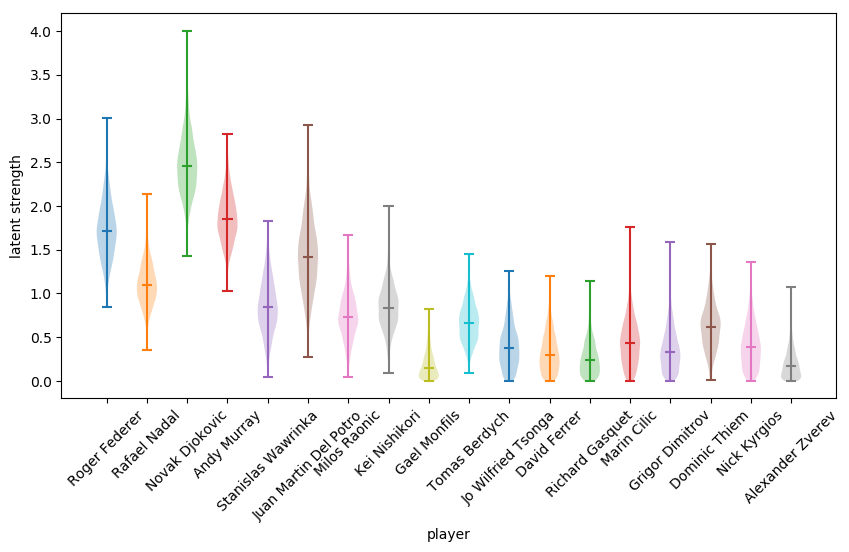
\includegraphics[clip,width=12.0cm]{./graphs/strength_mu.png}
    \caption{各プレイヤーの強さ $\mu_n$ の事後分布の中央値, 不偏標準偏差, 50\%ベイズ信用区間の下限および上限}
    \label{tb:tb_strength_mu}
  \end{center}
\end{table}
 %ヴァイオリンプロットが各プレイヤーの強さ $\mu_n$ のプロット, 表はそれぞれの中央値, 50\%ベイズ信頼区間の下限、上限である。\\
 対象期間は「ジョコビッチ1強時代」と言われていたほどであり, 結果を確認しても, ジョコビッチが1番強いという直感通りの結果となった。\\
 デル・ポトロもBIG4に引けを取らない強さとなっているが, 怪我などの影響で勝負回数が少ないからか, 帯も大きく伸びていて不確実度が高いことが分かる。\\
 錦織はワウリンカと同じくらいの強さとなっている。この時すでにグランドスラムを*回制しているワウリンカの方が強いのではないかと予想していたが, 意外な結果となった。\\
 表*に, 対象期間中の勝ちプレイヤー(行)・負けプレイヤー(列)であった試合数をマス目の数値で表した戦績表を記す。\\
\begin{table}[htbp]
  \begin{center}
    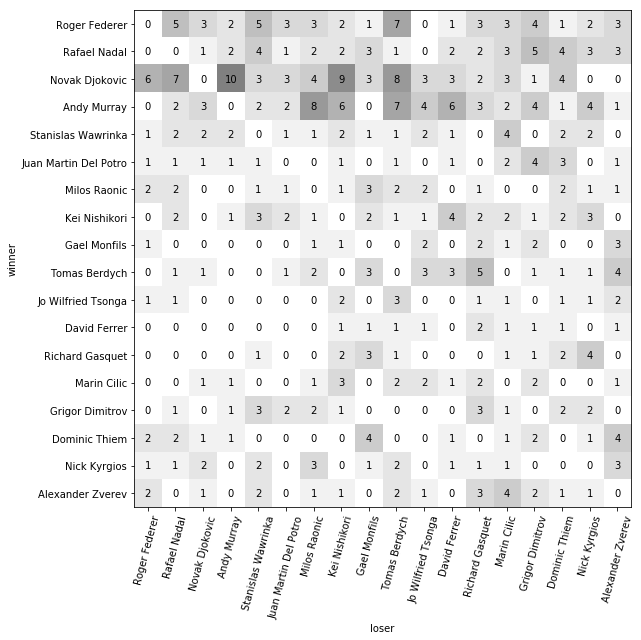
\includegraphics[clip,width=12.0cm]{./graphs/strength_winlose_crosstab.png}
    \caption{2015.01〜2017.02期間中の各プレイヤーの勝敗戦績}
    \label{tb:tb_strength_winlose_crosstab}
  \end{center}
\end{table}
 これを見ても確かに, 対象期間中では, 錦織はワウリンカに3勝2敗で勝ち越しており, ワウリンカ, 錦織共にBIG4相手に白星を上げていることもあるため, 改めて錦織がTop10の中でも強い部類に位置していることを確認できた。\\
 また, 対象期間中では, 若手プレイヤーは中堅以上のプレイヤーに対しては若干劣る様子で, 若手の中では, ティエムが強いという結果となった。\\
 続いて, 勝負ムラ ${\sigma_{pf}}_n$ の事後分布を図*, 表*に記す。\\
\begin{figure}[htbp]
  \begin{center}
    
\includegraphics[clip,width=12.0cm]{./graphs/strength_s_pf.png}
    \caption{各プレイヤーの勝負ムラ ${\sigma_{pf}}_n$ の事後分布のヴァイオリンプロット}
    \label{fig:fig_strength_s_pf}
  \end{center}
\end{figure}
\begin{table}[htbp]
  \begin{center}
    
\includegraphics[clip,width=12.0cm]{./graphs/strength_s_pf.png}
    \caption{各プレイヤーの勝負ムラ ${\sigma_{pf}}_n$ の事後分布の中央値, 不偏標準偏差, 50\%ベイズ信用区間の下限および上限}
    \label{tb:tb_strength_s_pf}
  \end{center}
\end{table}
 確認してみると, ワウリンカが勝負ムラが一番大きいという結果となった。戦績表*を確認すると確かに, BIG4に限らず, 同じプレイヤー相手に勝ったり負けたりしていることがよくわかる。\\
 BIG4の中では, 対象期間中では, 若干フェデラー, ナダルが勝ったり負けたりしているため, 勝負ムラが少し大きめに出ている。\\
 チリッチもこの期間では, ジョコビッチ, マレーに勝ったことがあり, その他選手とも勝ったり負けたりが多く, 結果, 勝負ムラが大きく出ている。\\
 個人的に面白いと思ったのは, 若手選手の勝負ムラが全体的に少し高めに出ていることで, まだパフォーマンスを安定して発揮することに慣れていないということが表されているのか, 興味深い結果となった。\\
 
\subsection{プロテニスプレイヤーの時系列で見た強さのモデル}
\subsubsection{モデルの仮定}
 前節では, 対象期間を定めた上で, 各プレイヤーの強さをモデリングすることができた。しかし, やはり時系列で各プレイヤーの強さがどのように推移してきたのかを見てみたい。\\
 そこで, 式(1)のモデルを以下のように拡張してみた。\\

\begin{eqnarray}
  {performance_{g,1}}_y & {\sim} & Normal(\mu_{loser,y},{\sigma_{pf}}_{loser,y}), \hspace{1em} g=1{\ldots}G, \hspace{0.5em} y=1{\ldots}Y \nonumber \\
  {performance_{g,2}}_y & {\sim} & Normal(\mu_{winner,y},{\sigma_{pf}}_{winner,y}), \hspace{1em} g={\ldots}G, \hspace{0.5em} y=1{\ldots}Y \nonumber \\
  {performance_{g,1}}_y & < & {performance_{g,2}}_y, \hspace{1em} g=1{\ldots}G, \hspace{0.5em} y=1{\ldots}Y \nonumber \\
  \mu_{n,1} & {\sim} & Normal(0,{\sigma_\mu}_{n,1}), \hspace{1em} n=1{\ldots}N \\
  \mu_{n,y} & {\sim} & Normal(\mu_{n,y-1},{\sigma_\mu}_{n,y-1}), \hspace{1em} n=1{\ldots}N,\hspace{0.5em} y=2{\ldots}Y \nonumber \\
  {\sigma_{pf}}_{n,y} & {\sim} & Gamma(10,10), \hspace{1em} n=1{\ldots}N,\hspace{0.5em} y=1{\ldots}Y \nonumber \\
  {\sigma_{\mu}}_{n,y} & {\sim} & Normal(0,1), \hspace{1em} n=1{\ldots}N,\hspace{0.5em} y=1{\ldots}Y \nonumber
  \label{eq:eq_strength_ts}
\end{eqnarray}

 考え方としては, $loser$ は負けたプレイヤーのインデックス, $winner$ は勝ったプレイヤーのインデックスを表すとし, プレイヤーの $y$ 年の強さを $\mu_{n,y}$, 勝負ムラを${\sigma_{pf}}_{n,y}$として, $y$ 年に行われる勝負で発揮する力(パフォーマンス)は, 平均$\mu_{n,y}$, 標準偏差 ${\sigma_{pf}}_{n,y}$ の正規分布から生成されると考える。勝負の結果はパフォーマンスの大小で決まるとする。プレイヤーの $y$ 年での強さ $\mu_{n,y}$ は, その1つ前の年の強さ$\mu_{n,y-1}$ から生成されると考える。\\
 また, 識別可能にするため, 以下の仮定を加えた。

\begin{table}[htb]
  \begin{tabular}{l}
    仮定1: 各プレイヤーの初年度の強さは, 平均0, 標準偏差 ${\sigma_{pf}}_{n,1}$ の半正規分布に従うとする \\
    仮定2: 各プレイヤーの年度別の強さの変化具合は ${\sigma_{\mu}}_{n,y}$ は半正規分布に従うとする
  \end{tabular}
\end{table}

 ここで仮定2は, 弱情報事前分布である。無情報事前分布でも試してみたが, 筆者の場合は収束しなかった。この部分は, 年を跨いだ時のプレイヤーの強さの変化のしやすさを表しているため, 次の年には別人のようにいきなり強くなるということは滅多に起きないだろうとし, この程度の仮定はあっても問題ないと判断した。\\
 対象期間は, 2005.01〜2016.12の戦績データを利用する。この期間だと, 前節での若手選手などはほとんどデータが足りなくなるため, 改めて対象プレイヤーを以下の通りに選択した。

\begin{table}[htb]
  \begin{tabular}{lll}
    Roger Federer & Milos Raonic & Richard Gasquet \\
    Rafael Nadal & Kei Nishikori & Marin Cilic \\
    Novak Djokovic & Gael Monfils & Grigor Dimitrov \\
    Andy Murray & Tomas Berdych & Dominic Thiem \\
    Stanislas Wawrinka & Jo Wilfried Tsonga & Nick Kyrgios \\
    Juan Martin Del Potro & David Ferrer & Alexander Zverev \\
  \end{tabular}
\end{table}

\subsubsection{プロテニスプレイヤーの時系列で見た強さの推定結果と考察}

 収束は前節と同様, Rhat統計量の方法で確認した。\\
 各プレイヤーの強さの時系列の推移を可視化してみる。\\
 まずはジョコビッチ, 錦織の強さの時系列の推移を, 中央値と25\%, 75\%あああああああああああ

\begin{figure}[htbp]
  \begin{center}
    %\includegraphics[clip,width=7.0cm]{./***.eps}
    \caption{グラフ8}
    %\label{fig:fig8}
  \end{center}
\end{figure}

 あああああああああああ
 改めて、各プレイヤーの強さの時系列の推移を中央値のみで以下に可視化してみる。

\begin{figure}[htbp]
  \begin{center}
    %\includegraphics[clip,width=7.0cm]{./***.eps}
    \caption{グラフ9}
    %\label{fig:fig9}
  \end{center}
\end{figure}

 筆者の感覚としては, 割と納得のいく推移結果が得られた。 \\
 2005年頃は, やはりフェデラー・ナダルの2強時代であった様子がよく分かる。 \\
 そして, 2008頃から, フェデラー・ナダルに迫る, 当時若手であったジョコビッチ, マレー, デル・ポトロの強さが上位に推移してきている。\\
 錦織は2014年に強さが急激に上昇しており, この年に初めて世界ランクTOP10入りをした。\\
 デル・ポトロは初めてグランドスラムを優勝した2009年に, 強さが上昇するものの, 怪我の影響で, その後の推移を落としている様子が伺える。\\
 マレーもかなりジグザグしているが, 2008年頃からフェデラー・ナダルに勝つようになり, この頃に世界ランク2位まで上り詰めるものの, 2014年に怪我で不調となっているため, そのような様子がはっきりと現れている。
 続いて, 各プレイヤーの各年ごとの勝負ムラの事後分布を可視化してみる。

\begin{figure}[htbp]
  \begin{center}
    %\includegraphics[clip,width=7.0cm]{./***.eps}
    \caption{グラフ10}
    %\label{fig:fig10}
  \end{center}
\end{figure}

 マレーが年によって勝負ムラが大きくなるような結果となった。\\
 ワウリンカは, 前節での分析では, 勝負ムラが大きかったものの, それまでの年で言えば, 比較的大きくはなかったようである。\\
 錦織は, 前節での分析と同様, 各年においても勝負ムラはあまり大きくない傾向にあり, 勝つ相手には勝つ, 負ける相手には負けるといったところがはっきりしているようである。\\
 最後に, 各プレイヤーの各年ごとの強さの成長の変化度合いの事後分布を可視化してみる。

\begin{figure}[htbp]
  \begin{center}
    %\includegraphics[clip,width=7.0cm]{./***.eps}
    \caption{グラフ11}
    %\label{fig:fig11}
  \end{center}
\end{figure}

 基本的には, 強さの時系列のモデルの傾きと, 大きさが連動している様子が伺える。\\
 初年の強さを0から推定させていることもあり, 元から強かったフェデラー・ナダルがいきなり強くなっているように見えるため, この辺りは無視した方が良さそうである。\\
 マレーは, フェデラー, ナダルに勝つようになった上向きの強さの変化と, 不調による下向きの強さの変化があったことが確認できる。\\
 他のプレイヤーも時系列と同様, デル・ポトロは2009年で強さが大きく変化している, 錦織は2014年で強さが大きく変化していることがグラフから確認できた。

\subsubsection{まとめ}

\subsubsection{付録}

本章で使用したStanコードを以下に記す。

\vspace{1em}

\begin{itembox}[l]{プロテニスプレイヤーの強さのモデル}
  \begin{verbatim}
data {
  int N;
  int G;
  int<lower=1, upper=N> LW[G, 2];
}
parameters {
  ordered[2] performance[G];
  vector<lower=0>[N] mu;
  real<lower=0> s_mu; 
  vector<lower=0>[N] s_pf;
}
model {
  for (g in 1:G)
    for (i in 1:2)
      performance[g, i] ~ normal(mu[LW[g, i]], s_pf[LW[g, i]]);
        
  mu ~ normal(0, s_mu);
  s_pf ~ gamma(10, 10);
}
  \end{verbatim}
  \label{cd:cd_model_strength}
\end{itembox}

\vspace{1em}

\begin{itembox}[l]{プロテニスプレイヤーの時系列で見た強さのモデル}
  \begin{verbatim}
data {
  int N;
  int G;
  int Y;
  int<lower=1> GY[G];
  int<lower=1, upper=N> LW[G, 2];
}
parameters {
  ordered[2] performance[G];
  matrix<lower=0>[N, Y] mu;
  matrix<lower=0>[N, Y] s_mu;
  matrix<lower=0>[N, Y] s_pf;
}
model {
  for (g in 1:G)
    for (i in 1:2)
      performance[g, i] ~ normal(mu[LW[g, i], GY[g]], s_pf[LW[g, i], GY[g]]);
        
  for (n in 1:N)
    mu[n, 1] ~ normal(0, s_mu[n, 1]);
            
  for (n in 1:N)
    for (y in 2:Y)
      mu[n, y] ~ normal(mu[n, y-1], s_mu[n, y]);
           
  for (n in 1:N)
    s_mu[n] ~ normal(0, 1);
        
  for (n in 1:N)
    s_pf[n] ~ gamma(10, 10);
}
  \end{verbatim}
  \label{cd:cd_model_strength_ts}
\end{itembox}
\vspace{0.5em}

\end{document}
